\chapter{Introducción biológica}
Este capítulo tiene por objetivo el introducir al lector en los conceptos biológicos básicos necesarios para comprender y motivar los datos presentados y analizados en este trabajo. El lector que desee profundizar sobre los mismos puede remitirse a \cite{Domany2003, Alberts2015}.
\section{Información hereditaria: ADN}
Las células y los organismos pueden ser divididos en dos ramas, procariotas (como las bacterias) y eucariotas (como las plantas, hongos y animales). En las procariotas, el material genético no ocupa una región definida dentro de la célula, sino que se encuentra disperso en el citoplasma, mientras que en las eucariotas, el material genético se encuentra separado del citoplasma en una región denominada núcleo (figura \ref{fig:celula_eucariota}).\\\\
Todas la células vivas de La Tierra transmiten su información genética hereditaria por medio del ADN (ácido desoxirribonucleico). El ADN es una molécula unidimensional formada por dos hebras enrolladas una alrededor de la otra en una estructura de doble hélice (figura \ref{fig:adn1}). Las hebras son cadenas largas de polímeros formadas por monómeros (los nucleótidos), que consisten en dos partes: una columna conformada por un azúcar (desoxirribosa) con un grupo fosfato adherido, y una base nitrogenada, que puede ser adenina (A), guanina (G), citosina (C) o timina (T). Cada azúcar se conecta al siguiente mediante un grupo fosfato, con una protuberancia formada por la base, creando de esta manera una cadena polimérica. 
\begin{figure}[h]
    \centering
    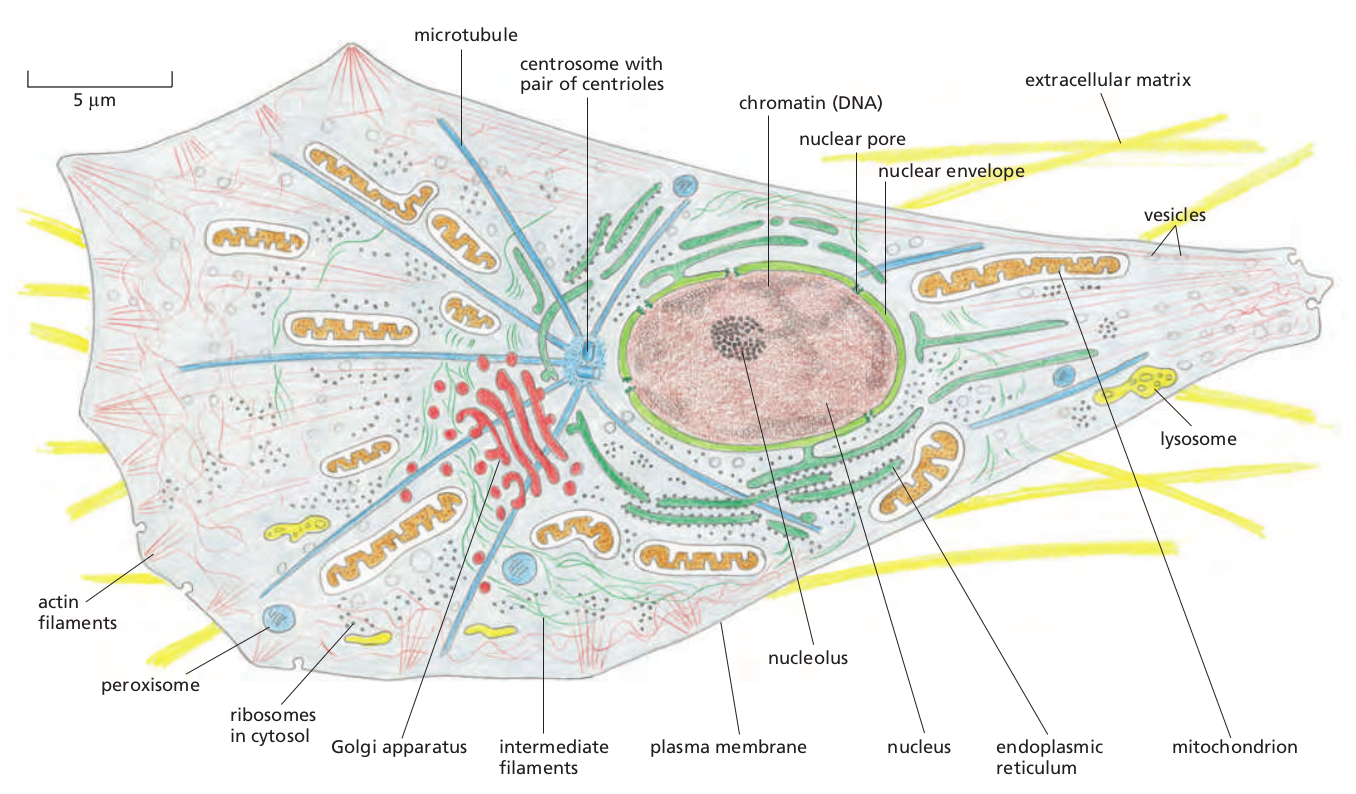
\includegraphics[width=0.8\textwidth]{celula_eucariota}
    \caption{La célula eucariota y sus principales características, entre las que se destacan los ribosomas y el núcleo conteniendo al ADN. (Fuente: Alberts \cite{Alberts2015})}
    \label{fig:celula_eucariota}
\end{figure}
En principio, es posible extender la cadena de ADN agregando cualquier monómero al final de la misma. Sin embargo, el ADN no se sintetiza como una única hebra, sino a partir de una hebra preexistente, por lo que cada nucléotido debe conectarse mediante puentes de hidrógeno con un nucléotido de la hebra preexistente siguiendo unas reglas estrictas definidas por la estructura complementaria de las bases: A se conecta con T (mediante dos puentes de hidrógeno) y C con G (mediante tres). De esta manera, se forma la estructura de doble hélice con hebras complementarias del ADN. Las uniones entre las bases son mucho más débiles que entre los azucares y los grupos fosfato, lo que permite a las hebras separarse sin que se rompan.\\\\
\begin{figure}[h]
    \centering
    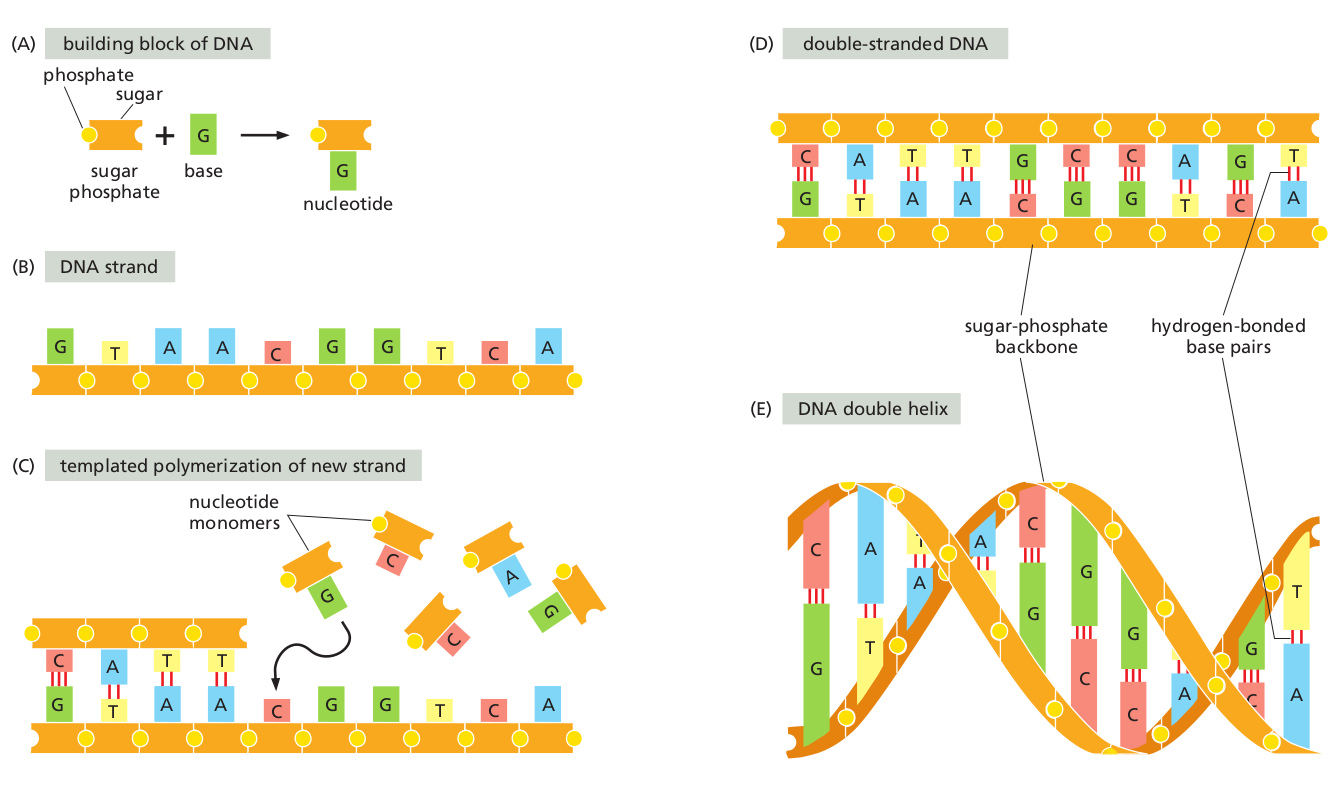
\includegraphics[width=0.8\textwidth]{adn1}
    \caption{Información hereditaria en el ADN. (A) Bloques constitutivos del ADN, esqueleto azúcar-fosfato y base nitrogenada. (B) Una hebra de ADN compuesta por el esqueleto de azucares-fosfatos y las bases. (C) Polimerización de una hebra a partir de otra que funciona como plantilla. (D) ADN completo con las dos hebras. (E) Forma final del ADN con las hebras en configuración de dóble hélice. (Fuente: Alberts \cite{Alberts2015})}
    \label{fig:adn1}
\end{figure}
Un gen es un segmento de ADN que contienen la información necesaria para la síntesis de una proteína en particular. Las proteínas son las moléculas que llevan a cabo casi todos los procesos dentro de una célula, y están compuestas por hasta 20 aminoácidos diferentes. Un gen es por lo tanto una receta que indica el orden en que se colocarán estos aminoácidos, codificada en la secuencia lineal de bases en la molécula de ADN. El genoma es la colección de todos los genes que codifican todas las proteínas que un organismo requiere para vivir. El genoma de un organismo sencillo como el de la levadura contiene alrededor de 6000 genes, mientras que el del humano contiene entre 30000 y 40000. La mayor parte del ADN humano (un 98\%) contiene regiones no codificantes, es decir, hebras que no codifican ninguna proteína en particular. Aunque en un principio se pensaba que esta enorme proporción del genoma no cumplía funcionalidad alguna (se hablaba del genoma basura o ``garbage genome'' en inglés), estudios recientes sugieren que, al menos en algunos casos, podría jugar un rol regulatorio en la síntesis de ciertas proteínas.\\\\

\section{Transcripción y traducción: dogma central de la biología molecular}
Para poder llevar a cabo la función de transmitir información, el ADN debe poder hacer algo más que replicarse. Debe poder expresar esa información que permite la síntesis de otras polímeros: el ARN y las proteínas.\\\\
El proceso para la síntesis de una proteína se conoce como transcripción y comienza con la síntesis de una molécula más corta de un polímero llamado ARN (ácido ribonucléico). En el ARN, la columna está conformada por el azucar ribosa y cuatro bases, uracilo (U) en lugar de timina, y las otras tres bases A, C y G son las mismas que en el ADN, apareándose cada una con su respectiva base complementaria. Durante la transcripción, las hebras de ADN se separan en la región a ser copiada y los monómeros que conforman el ARN son conectados con sus bases complementarias en el ADN (figura \ref{fig:adn2}).\\ 
\begin{figure}[h]
    \centering
    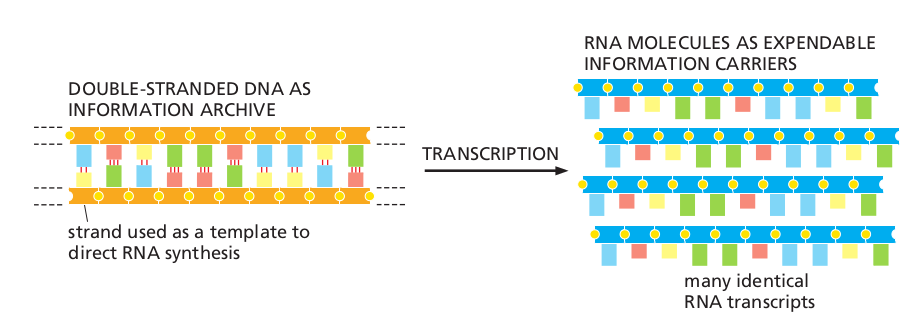
\includegraphics[width=0.8\textwidth]{adn2}
    \caption{Proceso de transcripción de información genética. Lo doble hebra del ADN se separa y cada hebra sirve como plantilla para la síntesis de ARN. (Fuente: Alberts \cite{Alberts2015})}
    \label{fig:adn2}
\end{figure}
La molécula de ARN final es una secuencia que reproduce fielmente la información del gen copiado, donde cada triplete de bases consecutivas (llamados codones) codifica cada aminoácido de la proteína a sintetizar, y es esta molécula la que es exportada desde el núcleo al citoplasma en forma de ARN mensajero (ARNm), dejando la información original intacta dentro del núcleo celular.\\\\
Esta molécula de ARNm será luego utilizada por el ribosoma, una maquinaria catalítica compleja consistente en más de 50 proteínas ribosomales diferentes y varias moléculas de ARN ribosomal, para sintetizar la proteína codificada por el gen, en un proceso llamado traducción. Todo el proceso completo de transcripción y traducción se conoce como dogma central de la biología molecular.
\begin{figure}[h]
    \centering
    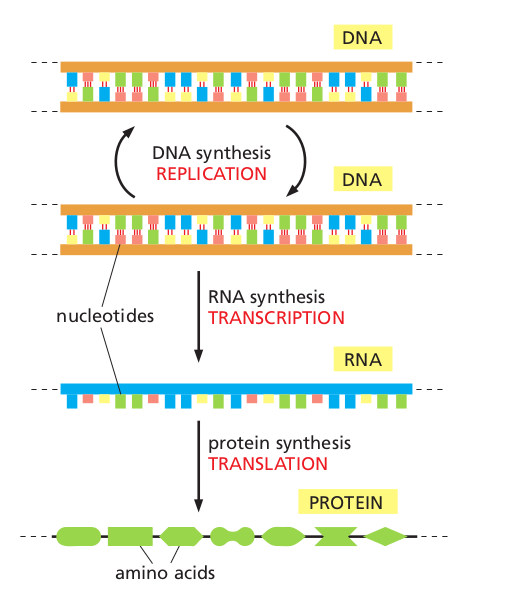
\includegraphics[width=0.5\textwidth]{adn3}
    \caption{Proceso de transcripción y traducción de información genética: dogma central de la biología molecular. El ADN se replica, se transcribe a ARN y luego se traduce a una proteína. (Fuente:Alberts \cite{Alberts2015})}
    \label{fig:adn3}
\end{figure}
Si bien cada célula que compone un organismo complejo posee el mismo ADN, células tomadas de distintos órganos realizan diferentes funciones, al igual que las proteínas en los mismos. Por ejemplo, las células de la retina requieren moléculas fotosensibles, mientras que las células que componen el hígado no las requieren. Existe entonces un proceso conocido como diferenciación dentro de cada célula. En lugar de sintetizar todas las posibles proteínas, la célula regula los niveles de transcripción y traducción de los genes que codifican las proteínas necesarias para la misma y únicamente esas proteínas son las que serán sintetizadas.\\\\
En un dado momento, la célula puede requerir muchas proteínas de un tipo y pocas de otro, es decir, en un dado momento cada gen individual puede expresarse a niveles diferentes. La transcripción de un gen (la orden de comenzar a copiarlo o de finalizar la copia) es regulada por proteínas especiales llamadas factores de transcripción, que se ligan a regiones específicas del ADN fuera de la región codificante, que inician o suprimen la transcripción. Esto lleva a la asunción en que se basa el análisis de expresión genética: el estado biológico de una célula queda determinado por su perfil de expresión, es decir, los niveles de expresión de cada gen individual en el genoma, que pueden ser inferidos a partir de las concentraciones de ARNm.\\\\
Conocer cuales son los genes que se expresan frente a determinados estímulos, puede brindar información sobre la función que realizan las proteínas codificadas por los mismos en el organismo, información clave para comprender las bases de enfermedades complejas como el cáncer.